\documentclass[12pt, a4paper]{article}

% ── Packages ──
\usepackage[margin=1in]{geometry}
\usepackage{amsmath, amssymb, amsfonts}
\usepackage{booktabs}
\usepackage{graphicx}
\usepackage{xcolor}
\usepackage{tikz}
\usetikzlibrary{calc, positioning, arrows.meta, decorations.pathreplacing}
\usepackage{tcolorbox}
\tcbuselibrary{skins, breakable}
\usepackage{enumitem}
\usepackage{hyperref}
\usepackage{fancyhdr}
\usepackage{titlesec}
\usepackage{float}
\usepackage{pifont}

% ── Colors ──
\definecolor{darkblue}{HTML}{1a365d}
\definecolor{medblue}{HTML}{2b6cb0}
\definecolor{lightblue}{HTML}{ebf8ff}
\definecolor{darkgreen}{HTML}{276749}
\definecolor{lightgreen}{HTML}{f0fff4}
\definecolor{darkred}{HTML}{9b2c2c}
\definecolor{lightred}{HTML}{fff5f5}
\definecolor{darkorange}{HTML}{c05621}
\definecolor{lightorange}{HTML}{fffaf0}
\definecolor{darkpurple}{HTML}{553c9a}
\definecolor{lightpurple}{HTML}{faf5ff}
\definecolor{darkteal}{HTML}{285e61}
\definecolor{lightteal}{HTML}{e6fffa}

% ── tcolorbox styles ──
\newtcolorbox{eqbox}[1][]{
    colback=lightpurple, colframe=darkpurple, fonttitle=\bfseries,
    title={#1}, rounded corners, boxrule=1pt, breakable
}
\newtcolorbox{explainbox}[1][]{
    colback=lightblue, colframe=medblue, fonttitle=\bfseries,
    title={#1}, rounded corners, boxrule=1pt, breakable
}
\newtcolorbox{examplebox}[1][]{
    colback=lightgreen, colframe=darkgreen, fonttitle=\bfseries,
    title={#1}, rounded corners, boxrule=1pt, breakable
}
\newtcolorbox{analogybox}[1][]{
    colback=lightorange, colframe=darkorange, fonttitle=\bfseries,
    title={#1}, rounded corners, boxrule=1pt, breakable
}
\newtcolorbox{warningbox}[1][]{
    colback=lightred, colframe=darkred, fonttitle=\bfseries,
    title={#1}, rounded corners, boxrule=1pt, breakable
}
\newtcolorbox{summarybox}[1][]{
    colback=lightteal, colframe=darkteal, fonttitle=\bfseries,
    title={#1}, rounded corners, boxrule=1pt, breakable
}

% ── Header/Footer ──
\pagestyle{fancy}
\fancyhf{}
\fancyhead[L]{\small\textcolor{darkblue}{Thesis Equations --- Explained}}
\fancyhead[R]{\small\textcolor{darkblue}{Reference Guide}}
\fancyfoot[C]{\thepage}
\renewcommand{\headrulewidth}{0.5pt}
\setlength{\headheight}{14pt}

% ── Section formatting ──
\titleformat{\section}{\LARGE\bfseries\color{darkblue}}{}{0em}{}[\vspace{-0.5em}\textcolor{medblue}{\rule{\textwidth}{1pt}}]
\titleformat{\subsection}{\Large\bfseries\color{medblue}}{}{0em}{}

\begin{document}

% ══════════════════════════════════════════════════════════════
%                        TITLE PAGE
% ══════════════════════════════════════════════════════════════
\begin{titlepage}
\centering
\vspace*{2cm}
{\Huge\bfseries\textcolor{darkblue}{Every Mathematical Equation}}\\[0.6cm]
{\Huge\bfseries\textcolor{darkblue}{in the Thesis --- Explained}}\\[1.5cm]
{\Large\textcolor{medblue}{A Symbol-by-Symbol Breakdown}}\\[0.5cm]
{\large\textcolor{medblue}{From Spatiotemporal Tokenization to HAF-STD Net}}\\[3cm]

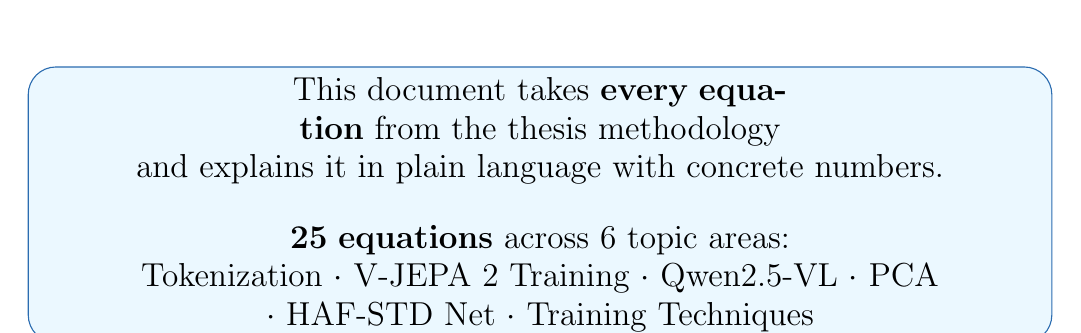
\begin{tikzpicture}
    \node[draw=medblue, fill=lightblue, rounded corners=10pt, minimum width=13cm, minimum height=3.5cm, text width=12cm, align=center, font=\large] {
        This document takes \textbf{every equation} from the thesis methodology\\
        and explains it in plain language with concrete numbers.\\[0.4cm]
        \textbf{25 equations} across 6 topic areas:\\
        Tokenization $\cdot$ V-JEPA 2 Training $\cdot$ Qwen2.5-VL $\cdot$ PCA\\
        $\cdot$ HAF-STD Net $\cdot$ Training Techniques
    };
\end{tikzpicture}

\vfill
{\large\today}
\end{titlepage}

\tableofcontents
\newpage

% ══════════════════════════════════════════════════════════════
%         PART 1: V-JEPA 2 --- SPATIOTEMPORAL TOKENIZATION
% ══════════════════════════════════════════════════════════════
\section{V-JEPA 2: Turning Video into Tokens}

\subsection{Equation 1 --- Spatiotemporal Tokenization (Eq.~3.1)}

\begin{eqbox}[The Equation]
\[
\mathbf{z}_0 = \text{Conv3D}(\mathbf{V}) + \mathbf{E}_{\text{pos}}, \quad \mathbf{z}_0 \in \mathbb{R}^{N \times D}
\]
\end{eqbox}

\begin{explainbox}[What Every Symbol Means]
\begin{tabular}{lp{11cm}}
$\mathbf{V}$ & The raw input video. It has shape $\mathbb{R}^{T \times H \times W \times 3}$, meaning $T$ frames, each of height $H$, width $W$, with 3 color channels (RGB). In your thesis: $T=8$, $H=W=224$, so $\mathbf{V}$ is an $8 \times 224 \times 224 \times 3$ tensor. \\[0.3cm]
$\text{Conv3D}(\cdot)$ & A 3D convolution operation. It slides a small 3D filter (size $2 \times 16 \times 16$) over the video volume. This filter groups 2 consecutive frames and a $16\times16$ spatial patch into one ``tubelet.'' Each tubelet is converted into a single vector. \\[0.3cm]
$\mathbf{E}_{\text{pos}}$ & Positional embeddings --- extra information added to tell the model \textit{where} each token comes from (its position in time and space). Uses 3D Rotary Position Embedding (RoPE). \\[0.3cm]
$\mathbf{z}_0$ & The output: a sequence of token vectors. The entire video is now represented as $N$ vectors, each of dimension $D$. \\[0.3cm]
$N$ & Total number of tokens $= \frac{T}{2} \times \frac{H}{16} \times \frac{W}{16}$. \\[0.3cm]
$D$ & Dimension of each token vector. For ViT-Huge: $D = 1280$.
\end{tabular}
\end{explainbox}

\begin{examplebox}[Computing N with Your Actual Numbers]
\[
N = \frac{8}{2} \times \frac{224}{16} \times \frac{224}{16} = 4 \times 14 \times 14 = \mathbf{784 \text{ tokens}}
\]
So a single 8-frame video clip becomes a sequence of \textbf{784 vectors}, each of dimension \textbf{1280}.

The shape is: $\mathbf{z}_0 \in \mathbb{R}^{784 \times 1280}$
\end{examplebox}

\begin{analogybox}[Plain English Analogy]
\textbf{Think of it like cutting a book into sentences.}

The video is like a book with pictures. Conv3D cuts it into small rectangular ``chunks'' (tubelets). Each chunk covers a small spatial area ($16 \times 16$ pixels) over a short time window (2 frames). Each chunk is then summarized as a single 1280-number description vector.

The positional embedding $\mathbf{E}_{\text{pos}}$ is like page numbers and paragraph numbers --- it tells the model ``this chunk came from the top-left of frame 3'' so it knows the spatial and temporal arrangement.
\end{analogybox}

% ══════════════════════════════════════════════════════════════
%         PART 2: V-JEPA 2 --- DUAL ENCODER AND TRAINING
% ══════════════════════════════════════════════════════════════
\newpage
\section{V-JEPA 2: How It Learns (Training Objectives)}

\subsection{Equation 2 --- Exponential Moving Average / EMA (Eq.~3.2)}

\begin{eqbox}[The Equation]
\[
\bar{\theta} \leftarrow \tau \bar{\theta} + (1 - \tau) \theta, \quad \tau \in [0.996, 1.0)
\]
\end{eqbox}

\begin{explainbox}[What Every Symbol Means]
\begin{tabular}{lp{11cm}}
$\theta$ & The weights of the \textbf{context encoder} (x-Encoder). This encoder is trained normally with gradient descent --- it learns from mistakes.\\[0.3cm]
$\bar{\theta}$ & The weights of the \textbf{target encoder} (y-Encoder). This encoder is \textit{not} trained by gradients. Instead, its weights slowly follow $\theta$.\\[0.3cm]
$\tau$ & The ``momentum'' parameter (between 0.996 and 1.0). It controls how slowly $\bar{\theta}$ follows $\theta$.\\[0.3cm]
$\leftarrow$ & ``Update to'' --- the left side gets a new value computed from the right side.
\end{tabular}
\end{explainbox}

\begin{examplebox}[Numerical Example with $\tau = 0.999$]
Suppose one particular weight value is:
\begin{itemize}
    \item Context encoder weight: $\theta = 0.50$
    \item Target encoder weight (before update): $\bar{\theta}_{\text{old}} = 0.42$
\end{itemize}

After the EMA update:
\[
\bar{\theta}_{\text{new}} = 0.999 \times 0.42 + 0.001 \times 0.50 = 0.41958 + 0.0005 = 0.4201
\]

The target encoder barely changed! It moved from 0.42 to 0.4201 --- just 0.02\% toward $\theta$. This extreme slowness creates a \textbf{stable prediction target} that doesn't jump around during training.
\end{examplebox}

\begin{analogybox}[Why Do This?]
\textbf{Imagine a teacher and a student.}

The student (context encoder $\theta$) learns actively from exercises. The teacher (target encoder $\bar{\theta}$) slowly absorbs what the student learns. The teacher provides stable ``answer keys'' for the student to learn from. If the teacher changed as fast as the student, the ``answer keys'' would be unreliable and the student would be chasing a moving target.

Without EMA, both encoders could ``collapse'' --- they'd learn to output the same constant vector for every input (useless).
\end{analogybox}


\subsection{Equation 3 --- Vision Transformer Block (Eq.~3.3)}

\begin{eqbox}[The Equation]
\[
\mathbf{z}'_l = \text{MHSA}(\text{LN}(\mathbf{z}_{l-1})) + \mathbf{z}_{l-1}, \qquad
\mathbf{z}_l = \text{FFN}(\text{LN}(\mathbf{z}'_l)) + \mathbf{z}'_l
\]
\end{eqbox}

\begin{explainbox}[What Every Symbol Means]
\begin{tabular}{lp{11cm}}
$\mathbf{z}_{l-1}$ & Input to layer $l$ (output of the previous layer). A sequence of $N$ token vectors.\\[0.2cm]
$\text{LN}(\cdot)$ & Layer Normalization --- scales each token to have mean 0 and variance 1. Stabilizes training.\\[0.2cm]
$\text{MHSA}(\cdot)$ & Multi-Head Self-Attention --- each token ``looks at'' every other token to figure out which ones are relevant. This is how the model learns relationships between different parts of the video.\\[0.2cm]
$\mathbf{z}'_l$ & Intermediate result after attention + residual connection.\\[0.2cm]
$+ \mathbf{z}_{l-1}$ & \textbf{Residual (skip) connection} --- adds the original input back. This prevents the ``vanishing gradient'' problem in deep networks.\\[0.2cm]
$\text{FFN}(\cdot)$ & Feed-Forward Network --- two linear layers with a nonlinearity (GELU) in between. Transforms each token independently.\\[0.2cm]
$\mathbf{z}_l$ & Final output of layer $l$.
\end{tabular}
\end{explainbox}

\begin{analogybox}[What Happens in One Transformer Layer]
Two stages happen in sequence:

\textbf{Stage 1 (Attention):} Every token asks: ``Which other tokens should I pay attention to?'' A token representing the gymnast's hands might attend to tokens representing the balance beam. The output is a new version of each token that incorporates information from related tokens.

\textbf{Stage 2 (FFN):} Each token is individually transformed through a small neural network. This is where the model applies ``thinking'' --- combining the gathered information into a more useful representation.

The $+$ signs (residual connections) ensure information from earlier layers can flow through without being lost. V-JEPA 2 has 32 such layers ($L=32$ for ViT-Huge), so the video tokens get progressively refined through 32 rounds of attention + FFN.
\end{analogybox}


\subsection{Equation 4 --- V-JEPA 2 Training Objective (Eq.~3.4)}

\begin{eqbox}[The Equation]
\[
\underset{\theta,\,\phi,\,\Delta_y}{\text{minimize}} \quad \|P_\phi(\Delta_y, E_\theta(x)) - \operatorname{sg}(E_{\bar{\theta}}(y))\|_1
\]
\end{eqbox}

\begin{explainbox}[What Every Symbol Means]
\begin{tabular}{lp{11cm}}
$x, y$ & Two different ``views'' (augmented versions) of the same video clip.\\[0.2cm]
$E_\theta(x)$ & Context encoder processes the full unmasked view $x$. Produces representations for all visible tokens.\\[0.2cm]
$E_{\bar{\theta}}(y)$ & Target encoder processes the complete view $y$. Produces ``ground truth'' target representations.\\[0.2cm]
$\operatorname{sg}(\cdot)$ & \textbf{Stop-gradient operator}. This is crucial --- it means ``use this value but do NOT send gradients back through it.'' The target encoder is only updated by EMA (Eq.~3.2), never by gradient descent.\\[0.2cm]
$\Delta_y$ & Learnable mask tokens that tell the predictor which spatial/temporal positions were masked out.\\[0.2cm]
$P_\phi(\cdot)$ & Predictor network --- a smaller transformer that takes the context encoder's output and the mask positions, and tries to predict what the target encoder would output for the masked regions.\\[0.2cm]
$\|\cdot\|_1$ & $L_1$ norm (absolute value of differences, summed). Measures how ``far apart'' the prediction is from the target.\\[0.2cm]
$\theta, \phi$ & Trainable parameters of the context encoder and predictor, respectively.
\end{tabular}
\end{explainbox}

\begin{analogybox}[The Core Idea of V-JEPA 2]
\textbf{``Fill in the blanks'' for video.}

Imagine you cover up 75\% of a video (random spatiotemporal patches). The model must \textbf{predict what the hidden parts look like} --- not at the pixel level, but in a learned abstract representation space. It's like asking: ``Given the gymnast's position in frames 1--4, what would frames 5--8 look like in concept?''

The key insight: by learning to predict in \textbf{latent space} (not pixel space), the model learns \textit{semantic} features (``gymnast is flipping'') rather than low-level texture.
\end{analogybox}


\subsection{Equation 5 --- Dense Per-Token Prediction Loss (Eq.~3.5)}

\begin{eqbox}[The Equation]
\[
\mathcal{L}_{\text{predict}} = \frac{1}{|M|} \sum_{i \in M} \|P_\phi(E_\theta(x), \Delta_y)_i - \operatorname{sg}(E_{\bar{\theta}}(y)_i)\|_1
\]
\end{eqbox}

\begin{explainbox}[What This Adds Over Eq.~3.4]
\begin{tabular}{lp{11cm}}
$M$ & The set of all masked token indices (positions that were hidden).\\[0.2cm]
$|M|$ & Size of that set --- how many tokens were masked.\\[0.2cm]
$\sum_{i \in M}$ & Sum over each masked position individually.\\[0.2cm]
$(\cdot)_i$ & The subscript $i$ means ``the representation at token position $i$.''\\[0.2cm]
$\frac{1}{|M|}$ & Average over all masked positions --- so the loss doesn't depend on how many tokens were masked.
\end{tabular}

\textbf{The key difference from Eq.~3.4:} V-JEPA~2.1 computes the loss \textit{separately for each masked token}, then averages. This gives the model a \textbf{dense, per-position learning signal} --- every masked patch gets its own gradient, forcing fine-grained spatial understanding.
\end{explainbox}


\subsection{Equation 6 --- Context Loss (Eq.~3.6)}

\begin{eqbox}[The Equation]
\[
\mathcal{L}_{\text{context}} = \frac{1}{|C|} \sum_{j \in C} \lambda_d(j) \cdot \|E_\theta(x)_j - \operatorname{sg}(E_{\bar{\theta}}(y)_j)\|_1
\]
\end{eqbox}

\begin{explainbox}[What Every Symbol Means]
\begin{tabular}{lp{11cm}}
$C$ & The set of \textbf{visible} (unmasked) context token indices.\\[0.2cm]
$\lambda_d(j)$ & A distance-dependent weight. Visible tokens that are \textit{close} to masked regions get \textbf{higher weight}. Tokens far from any mask get lower weight.\\[0.2cm]
Purpose & This forces visible tokens near masked boundaries to have accurate representations too --- not just the masked ones.
\end{tabular}
\end{explainbox}

\subsection{Equation 7 --- Total V-JEPA 2.1 Loss (Eq.~3.7)}

\begin{eqbox}[The Equation]
\[
\mathcal{L}_{\text{V-JEPA~2.1}} = \mathcal{L}_{\text{predict}} + \lambda_d \cdot \mathcal{L}_{\text{context}}
\]
\end{eqbox}

\begin{explainbox}[Plain English]
The total training loss is the sum of two parts:
\begin{enumerate}
    \item $\mathcal{L}_{\text{predict}}$: How well can we predict the masked tokens? (primary task)
    \item $\lambda_d \cdot \mathcal{L}_{\text{context}}$: Are the visible tokens near masked regions also good? (auxiliary regularizer)
\end{enumerate}
$\lambda_d$ is a scalar weight that controls how much importance the context loss gets relative to the prediction loss.
\end{explainbox}


\subsection{Equation 8 --- Multi-Layer Feature Extraction (Eq.~3.8)}

\begin{eqbox}[The Equation]
\[
\mathbf{F}_{\text{multi}} = [\bar{\mathbf{z}}_{L/4};\; \bar{\mathbf{z}}_{L/2};\; \bar{\mathbf{z}}_{3L/4};\; \bar{\mathbf{z}}_{L}] \in \mathbb{R}^{4 \times T' \times D}
\]
\end{eqbox}

\begin{explainbox}[What Every Symbol Means]
\begin{tabular}{lp{11cm}}
$L$ & Total number of transformer layers (32 for ViT-Huge).\\[0.2cm]
$L/4, L/2, 3L/4, L$ & Layers 8, 16, 24, 32 --- features from 25\%, 50\%, 75\%, 100\% depth.\\[0.2cm]
$\bar{\mathbf{z}}_l$ & Features from layer $l$ after \textbf{spatial mean pooling} (averaging over the $14 \times 14 = 196$ spatial positions within each temporal frame). Shape: $\mathbb{R}^{T' \times D}$.\\[0.2cm]
$T'$ & Number of temporal tokens after tubelet grouping. $T' = T/2 = 8/2 = 4$ temporal positions.\\[0.2cm]
$[\cdot;\cdot;\cdot;\cdot]$ & Stacking the four layers together.\\[0.2cm]
$\mathbb{R}^{4 \times T' \times D}$ & Final shape: $4 \times 4 \times 1280$ = 4 layers $\times$ 4 time steps $\times$ 1280 dimensions.
\end{tabular}
\end{explainbox}

\begin{examplebox}[Concrete Shape]
$\mathbf{F}_{\text{multi}} \in \mathbb{R}^{4 \times 4 \times 1280}$

This is a 3D tensor with 20,480 numbers total. It contains features from 4 different depths of the network, at 4 different time points, each described by 1280 numbers. This is the input to the HAF-STD Net classifier.
\end{examplebox}

\begin{analogybox}[Why Multiple Layers?]
Early layers (layer 8) capture low-level features: edges, textures, simple motions.
Middle layers (16, 24) capture mid-level features: body parts, apparatus shapes.
Final layer (32) captures high-level semantic features: ``this is a vault'' vs ``this is a beam routine.''

By using \textbf{all four}, the HAF-STD Net gets a richer, multi-scale view of the video than any single layer alone.
\end{analogybox}


% ══════════════════════════════════════════════════════════════
%                    PART 3: QWEN2.5-VL
% ══════════════════════════════════════════════════════════════
\newpage
\section{Qwen2.5-VL: The Vision-Language Model}

\subsection{Equation 9 --- Patch Embedding (Eq.~3.9)}

\begin{eqbox}[The Equation]
\[
\mathbf{v}_0 = \text{Conv3D}(\mathbf{V}_{\text{frames}}), \quad \mathbf{v}_0 \in \mathbb{R}^{N_v \times D_v}
\]
\end{eqbox}

\begin{explainbox}[What Every Symbol Means]
\begin{tabular}{lp{11cm}}
$\mathbf{V}_{\text{frames}}$ & The input video frames (4 frames in this thesis).\\[0.2cm]
$\text{Conv3D}(\cdot)$ & 3D convolution that converts raw pixels into patch tokens. Uses $14 \times 14$ spatial patches and temporal stride of 2.\\[0.2cm]
$N_v$ & Number of visual tokens. Unlike V-JEPA 2 (fixed), this \textbf{varies dynamically} based on input resolution.\\[0.2cm]
$D_v$ & Hidden dimension of the vision encoder.
\end{tabular}

This is conceptually similar to V-JEPA's Eq.~3.1 but with a key difference: Qwen preserves the \textbf{original resolution} of each frame instead of resizing everything to $224 \times 224$.
\end{explainbox}


\subsection{Equation 10 --- Window Attention (Eq.~3.10)}

\begin{eqbox}[The Equation]
\[
\text{WindowAttn}(\mathbf{Q}, \mathbf{K}, \mathbf{V}) = \text{softmax}\!\left(\frac{\mathbf{Q}_w \mathbf{K}_w^T}{\sqrt{d_k}}\right) \mathbf{V}_w
\]
\end{eqbox}

\begin{explainbox}[What Every Symbol Means]
\begin{tabular}{lp{11cm}}
$\mathbf{Q}, \mathbf{K}, \mathbf{V}$ & Query, Key, Value matrices --- the three projections that every attention mechanism computes from input tokens. (Note: $\mathbf{V}$ here means ``Value,'' not ``video''!)\\[0.2cm]
$\mathbf{Q}_w, \mathbf{K}_w, \mathbf{V}_w$ & The subscript $w$ means these are restricted to tokens \textbf{within the same spatial window} (e.g., a $112 \times 112$ pixel region).\\[0.2cm]
$\mathbf{Q}_w \mathbf{K}_w^T$ & Matrix multiplication of queries with keys. This computes ``compatibility scores'' --- how much each token should attend to each other token.\\[0.2cm]
$\sqrt{d_k}$ & Scaling factor ($d_k$ = dimension of each key). Prevents the dot products from becoming too large, which would make softmax produce extreme (near-0 or near-1) values.\\[0.2cm]
$\text{softmax}(\cdot)$ & Converts raw scores into probabilities that sum to 1. Each token gets a probability distribution over which other tokens to attend to.\\[0.2cm]
$\cdot\; \mathbf{V}_w$ & Multiply the attention probabilities by the values. This produces a weighted average of the value vectors --- each token's output is a ``summary'' of the tokens it attended to.
\end{tabular}
\end{explainbox}

\begin{analogybox}[Why ``Window'' Attention?]
Standard (global) self-attention lets every token attend to \textbf{every} other token. With $N$ tokens, this requires $N^2$ computations --- quadratic scaling.

With 1000 tokens: $1000^2 = 1{,}000{,}000$ computations.\\
With 10,000 tokens: $10{,}000^2 = 100{,}000{,}000$ computations. Too expensive!

Window attention restricts each token to only attend within its local $w \times w$ window. Cost becomes $N \times w^2$ --- \textbf{linear in $N$}, not quadratic.
\end{analogybox}


\subsection{Equation 11 --- Multimodal Rotary Position Embedding / MRoPE (Eq.~3.11)}

\begin{eqbox}[The Equation]
\[
\text{MRoPE}(\mathbf{x}, t, h, w) = \mathbf{x} \odot \left[\cos(\theta_t), \cos(\theta_h), \cos(\theta_w)\right] + \hat{\mathbf{x}} \odot \left[\sin(\theta_t), \sin(\theta_h), \sin(\theta_w)\right]
\]
\end{eqbox}

\begin{explainbox}[What Every Symbol Means]
\begin{tabular}{lp{11cm}}
$\mathbf{x}$ & The input token vector.\\[0.2cm]
$t, h, w$ & Three position coordinates: time, height, width.\\[0.2cm]
$\theta_t, \theta_h, \theta_w$ & Rotation angles computed from each position coordinate. Different frequencies for different dimensions of the embedding.\\[0.2cm]
$\odot$ & Element-wise (Hadamard) multiplication --- multiply corresponding elements.\\[0.2cm]
$\hat{\mathbf{x}}$ & The ``rotated complement'' --- a rearranged version of $\mathbf{x}$ (pairs of dimensions are swapped with sign changes).\\[0.2cm]
$\cos, \sin$ & The trigonometric functions create a \textbf{rotation} in 2D subspaces of the embedding. Each pair of dimensions is rotated by an angle determined by position.
\end{tabular}
\end{explainbox}

\begin{analogybox}[What Rotary Position Embedding Does]
\textbf{Think of a clock.}

Standard position encoding adds a number (``you are token \#5''). RoPE instead \textbf{rotates} the token vector by an angle proportional to its position. When two tokens compute attention ($\mathbf{Q} \cdot \mathbf{K}$), the dot product naturally captures the \textbf{distance} between them (because rotation differences encode positional differences).

MRoPE extends this to \textbf{3 axes}: time, height, width. The embedding dimension is split into 3 groups, and each group is rotated based on one of the three coordinates. This lets the model understand both spatial and temporal position simultaneously.

Key insight: for pure text (no visual input), all three coordinates are set equal ($t = h = w$), which reduces MRoPE to standard 1D RoPE.
\end{analogybox}


\subsection{Equation 12 --- Visual-Language Fusion (Eq.~3.12)}

\begin{eqbox}[The Equation]
\[
\mathbf{v}_{\text{lang}} = \text{MLP}_{\text{merge}}(\mathbf{v}_{\text{enc}}), \quad \mathbf{v}_{\text{lang}} \in \mathbb{R}^{N_v' \times D_{\text{LM}}}
\]
\end{eqbox}

\begin{explainbox}[What Every Symbol Means]
\begin{tabular}{lp{11cm}}
$\mathbf{v}_{\text{enc}}$ & Visual tokens from the Vision Encoder (output of all the window attention layers).\\[0.2cm]
$\text{MLP}_{\text{merge}}$ & A Multi-Layer Perceptron (small neural network with 2--3 linear layers) that projects the vision tokens into the language model's space.\\[0.2cm]
$D_{\text{LM}} = 3584$ & The hidden dimension of the Qwen2.5 language model decoder. This is the ``language space.''\\[0.2cm]
$N_v'$ & Number of visual tokens after merging (may differ from $N_v$ if tokens are pooled/compressed).\\[0.2cm]
$\mathbf{v}_{\text{lang}}$ & The visual tokens now live in the same vector space as text tokens --- they can be mixed together.
\end{tabular}

\textbf{This is the bridge between vision and language.} After this projection, visual tokens and text tokens are interleaved into a single sequence and processed jointly by the language model decoder.
\end{explainbox}


\subsection{Equation 13 --- Language Model Training Objective (Eq.~3.13)}

\begin{eqbox}[The Equation]
\[
\mathcal{L}_{\text{LM}} = -\sum_{t=1}^{T_{\text{seq}}} \log p_\theta(x_t \mid x_{<t}, \mathbf{v}_{\text{lang}})
\]
\end{eqbox}

\begin{explainbox}[What Every Symbol Means]
\begin{tabular}{lp{11cm}}
$T_{\text{seq}}$ & Total length of the text sequence.\\[0.2cm]
$x_t$ & The $t$-th text token in the sequence.\\[0.2cm]
$x_{<t}$ & All text tokens before position $t$ (the ``history'').\\[0.2cm]
$\mathbf{v}_{\text{lang}}$ & The visual tokens (providing visual context).\\[0.2cm]
$p_\theta(x_t \mid x_{<t}, \mathbf{v}_{\text{lang}})$ & The model's predicted probability of token $x_t$ given all previous tokens and the visual input.\\[0.2cm]
$\log$ & Natural logarithm. Taking the log converts multiplication of probabilities into sums (numerically stable).\\[0.2cm]
$-$ & Negative sign makes it a loss to \textbf{minimize}. Minimizing the negative log-probability is equivalent to maximizing the probability of the correct next token.\\[0.2cm]
$\sum$ & Sum over all positions --- the model must predict every token correctly.
\end{tabular}

\textbf{In plain English:} The model is trained to predict the next word given the image and all previous words. This is standard autoregressive language model training.
\end{explainbox}


\subsection{Equation 14 --- NF4 Quantization (Eq.~3.14)}

\begin{eqbox}[The Equation]
\[
\mathbf{W}_{\text{NF4}} = \text{quantize}_{\text{NF4}}\!\left(\frac{\mathbf{W}}{s}\right) \cdot s, \quad s = \frac{\max(|\mathbf{W}_{\text{block}}|)}{q_{\max}}
\]
\end{eqbox}

\begin{explainbox}[What Every Symbol Means]
\begin{tabular}{lp{11cm}}
$\mathbf{W}$ & Original full-precision (float16) model weights.\\[0.2cm]
$\mathbf{W}_{\text{block}}$ & A small block of weights (e.g., 64 values). Quantization is done block-by-block, not globally.\\[0.2cm]
$s$ & Per-block \textbf{scaling factor}. It's the ratio of the maximum absolute value in the block to the maximum representable value in 4-bit.\\[0.2cm]
$\mathbf{W}/s$ & Normalized weights --- divided by $s$ to fit into the [-1, 1] range.\\[0.2cm]
$\text{quantize}_{\text{NF4}}(\cdot)$ & Maps each normalized value to the nearest of the 16 NF4 quantization levels ($2^4 = 16$ levels for 4-bit). These 16 levels are specifically chosen to minimize error for normally distributed values.\\[0.2cm]
$\cdot\; s$ & Multiply back by $s$ to restore the original scale.\\[0.2cm]
$q_{\max}$ & Maximum quantile value in the NF4 data type.
\end{tabular}
\end{explainbox}

\begin{examplebox}[Why This Matters: Memory Savings]
\textbf{Without quantization:} 7B parameters $\times$ 2 bytes (float16) = \textbf{14 GB}\\
\textbf{With NF4 (4-bit):} 7B parameters $\times$ 0.5 bytes = \textbf{3.5 GB} + scaling factors $\approx$ \textbf{4 GB total}

Your GPU has 15.6 GB. Without quantization, the model alone fills 14 GB, leaving almost no room for input data and intermediate computations. With NF4, the model takes only 4 GB, leaving 11.6 GB for actual work.
\end{examplebox}


\subsection{Equation 15 --- Qwen Feature Extraction (Eq.~3.15)}

\begin{eqbox}[The Equation]
\[
\mathbf{f}_{\text{Qwen}} = \frac{1}{T_{\text{seq}}} \sum_{t=1}^{T_{\text{seq}}} \mathbf{h}_t^{(L)}, \quad \mathbf{f}_{\text{Qwen}} \in \mathbb{R}^{3584}
\]
\end{eqbox}

\begin{explainbox}[What Every Symbol Means]
\begin{tabular}{lp{11cm}}
$\mathbf{h}_t^{(L)}$ & The hidden state vector at position $t$ from the \textbf{final} decoder layer $L$. Each is a 3584-dimensional vector.\\[0.2cm]
$T_{\text{seq}}$ & Total sequence length (visual tokens + text tokens combined).\\[0.2cm]
$\sum_{t=1}^{T_{\text{seq}}}$ & Sum over all positions in the sequence.\\[0.2cm]
$\frac{1}{T_{\text{seq}}}$ & Divide by the count to get the \textbf{average} (mean pooling).\\[0.2cm]
$\mathbf{f}_{\text{Qwen}}$ & The final feature vector for one video clip: a single vector of 3584 numbers.
\end{tabular}

\textbf{In plain English:} Take the last layer's output at every position, average them all together into one vector. This single 3584-d vector is the ``summary'' of the entire video clip.
\end{explainbox}


% ══════════════════════════════════════════════════════════════
%         PART 4: FROZEN FEATURE PROTOCOL & PCA
% ══════════════════════════════════════════════════════════════
\newpage
\section{Feature Preprocessing: Frozen Protocol and PCA}

\subsection{Equation 16 --- Frozen Feature Protocol}

\begin{eqbox}[The Equations]
\[
\mathbf{z}_i = f(\mathbf{x}_i; \mathbf{\Theta}_{\text{frozen}}), \quad \nabla_{\mathbf{\Theta}} \mathcal{L} = \mathbf{0}
\]
\[
\mathbf{W}_{\text{head}}^* = \arg\min_{\mathbf{W}_{\text{head}}} \frac{1}{N}\sum_{i=1}^{N} \mathcal{L}\left( g(\mathbf{z}_i; \mathbf{W}_{\text{head}}), y_i \right)
\]
\end{eqbox}

\begin{explainbox}[What Every Symbol Means]
\textbf{First equation:}
\begin{tabular}{lp{11cm}}
$\mathbf{x}_i$ & The $i$-th input video clip.\\[0.2cm]
$f(\cdot\,; \mathbf{\Theta}_{\text{frozen}})$ & The backbone model (V-JEPA 2 or Qwen2.5-VL) with frozen parameters. The semicolon means ``parameterized by.''\\[0.2cm]
$\mathbf{z}_i$ & The extracted feature vector for clip $i$.\\[0.2cm]
$\nabla_{\mathbf{\Theta}} \mathcal{L} = \mathbf{0}$ & ``The gradient of the loss with respect to $\mathbf{\Theta}$ is zero.'' This formally means: \textbf{we do not update the backbone weights}. No gradients flow through the backbone.
\end{tabular}

\textbf{Second equation:}
\begin{tabular}{lp{11cm}}
$g(\cdot\,; \mathbf{W}_{\text{head}})$ & The downstream classifier (SVM, MLP, HAF-STD Net, etc.) parameterized by $\mathbf{W}_{\text{head}}$.\\[0.2cm]
$y_i$ & True label for clip $i$.\\[0.2cm]
$\mathcal{L}(\cdot, \cdot)$ & Loss function (cross-entropy) comparing prediction with true label.\\[0.2cm]
$\frac{1}{N}\sum_{i=1}^{N}$ & Average loss over all $N$ training samples.\\[0.2cm]
$\arg\min$ & ``Find the $\mathbf{W}_{\text{head}}$ that minimizes this.''\\[0.2cm]
$\mathbf{W}_{\text{head}}^*$ & The optimal classifier weights after training.
\end{tabular}
\end{explainbox}

\begin{analogybox}[Why Freeze the Backbone?]
Think of the backbone (V-JEPA 2 / Qwen) as a \textbf{camera lens}. It was designed and calibrated at a factory (pretrained on millions of videos). You don't grind new glass for each photo shoot --- you just choose the right film (classifier) for the job.

Freezing has practical benefits: (1) saves GPU memory (no gradient storage), (2) prevents overfitting on small datasets, (3) enables fair comparison between different classifiers using the same fixed features.
\end{analogybox}


\subsection{Equation 17 --- Standardization (Eq.~3.16)}

\begin{eqbox}[The Equation]
\[
\tilde{\mathbf{z}}_{ij} = \frac{z_{ij} - \mu_j}{\sigma_j}, \quad \mu_j = \frac{1}{N_{\text{train}}} \sum_{i=1}^{N_{\text{train}}} z_{ij}, \quad \sigma_j = \sqrt{\frac{1}{N_{\text{train}}-1} \sum_{i=1}^{N_{\text{train}}} (z_{ij} - \mu_j)^2}
\]
\end{eqbox}

\begin{explainbox}[What Every Symbol Means]
\begin{tabular}{lp{11cm}}
$z_{ij}$ & Raw feature value for sample $i$, dimension $j$.\\[0.2cm]
$\mu_j$ & Mean of dimension $j$ computed over the training set. Add up all training samples' values for that dimension, divide by count.\\[0.2cm]
$\sigma_j$ & Standard deviation of dimension $j$. Measures how ``spread out'' the values are.\\[0.2cm]
$\tilde{\mathbf{z}}_{ij}$ & Standardized value. After transformation, dimension $j$ has mean $= 0$ and standard deviation $= 1$ across the training set.\\[0.2cm]
$N_{\text{train}}$ & Number of training samples (not test samples --- to avoid data leakage).\\[0.2cm]
$N_{\text{train}} - 1$ & Bessel's correction --- using $N-1$ instead of $N$ gives an unbiased estimate of the population variance.
\end{tabular}
\end{explainbox}

\begin{examplebox}[Numerical Example]
Suppose dimension $j = 42$ has these values across 5 training samples: $[10, 20, 30, 40, 50]$.

$\mu_{42} = \frac{10+20+30+40+50}{5} = 30$

$\sigma_{42} = \sqrt{\frac{(10-30)^2 + (20-30)^2 + \ldots + (50-30)^2}{5-1}} = \sqrt{\frac{400+100+0+100+400}{4}} = \sqrt{250} = 15.81$

The value $z_{1,42} = 10$ becomes: $\tilde{z}_{1,42} = \frac{10 - 30}{15.81} = -1.265$

Now all dimensions have the same scale, so dimension 42 (which ranged 10--50) and dimension 99 (which might range 0.001--0.005) are treated equally by PCA and the classifiers.
\end{examplebox}


\subsection{Equations 18--20 --- PCA (Eqs.~3.17--3.19)}

\begin{eqbox}[Covariance Matrix (Eq.~3.17)]
\[
\mathbf{C} = \frac{1}{N_{\text{train}}-1} \tilde{\mathbf{Z}}_{\text{train}}^\top \tilde{\mathbf{Z}}_{\text{train}} \in \mathbb{R}^{D \times D}
\]
\end{eqbox}

\begin{explainbox}[What This Does]
\begin{tabular}{lp{11cm}}
$\tilde{\mathbf{Z}}_{\text{train}}$ & The standardized feature matrix. Shape: $N_{\text{train}} \times D$ (samples $\times$ dimensions).\\[0.2cm]
$\tilde{\mathbf{Z}}_{\text{train}}^\top$ & Its transpose. Shape: $D \times N_{\text{train}}$.\\[0.2cm]
$\tilde{\mathbf{Z}}^\top \tilde{\mathbf{Z}}$ & Matrix multiplication. The result is a $D \times D$ matrix where entry $(i,j)$ measures how correlated dimensions $i$ and $j$ are.\\[0.2cm]
$\mathbf{C}$ & The covariance matrix. Diagonal entries = variance of each dimension. Off-diagonal entries = covariance (correlation) between pairs of dimensions.
\end{tabular}

For V-JEPA 2 ($D = 1280$): $\mathbf{C}$ is a $1280 \times 1280$ matrix with 1,638,400 entries.
\end{explainbox}

\begin{eqbox}[Variance Retention Threshold (Eq.~3.18)]
\[
k^* = \arg\min_{k} \left( \frac{\sum_{j=1}^{k} \lambda_j}{\sum_{j=1}^{D} \lambda_j} \ge 0.95 \right)
\]
\end{eqbox}

\begin{explainbox}[What This Does]
\begin{tabular}{lp{11cm}}
$\lambda_j$ & The $j$-th eigenvalue of $\mathbf{C}$, sorted in descending order. Each eigenvalue represents how much ``information'' (variance) the $j$-th principal component captures.\\[0.2cm]
$\sum_{j=1}^{k} \lambda_j$ & Total variance captured by the first $k$ components.\\[0.2cm]
$\sum_{j=1}^{D} \lambda_j$ & Total variance across all $D$ components.\\[0.2cm]
The ratio & The fraction of total variance captured by keeping only $k$ components.\\[0.2cm]
$\ge 0.95$ & We want at least 95\% of the information preserved.\\[0.2cm]
$k^*$ & The smallest $k$ that achieves this. This is how many dimensions we keep.
\end{tabular}
\end{explainbox}

\begin{examplebox}[Your Actual Results]
\begin{center}
\begin{tabular}{lccc}
\toprule
\textbf{Configuration} & \textbf{Original $D$} & \textbf{Reduced $k^*$} & \textbf{Compression Ratio} \\
\midrule
V-JEPA 2 on FineGym & 1,280 & 90 & $14.2\times$ \\
Qwen2.5-VL on FineGym & 3,584 & 142 & $25.2\times$ \\
V-JEPA 2 on HMDB51 & 1,280 & 286 & $4.5\times$ \\
Qwen2.5-VL on HMDB51 & 3,584 & 719 & $5.0\times$ \\
\bottomrule
\end{tabular}
\end{center}
HMDB51 needs more components because 51 classes require more information to distinguish than 4 classes.
\end{examplebox}

\begin{eqbox}[PCA Projection (Eq.~3.19)]
\[
\mathbf{Z}_{\text{PCA}} = \tilde{\mathbf{Z}} \, \mathbf{V}_{:k^*} \in \mathbb{R}^{N \times k^*}
\]
\end{eqbox}

\begin{explainbox}[What This Does]
\begin{tabular}{lp{11cm}}
$\tilde{\mathbf{Z}}$ & Standardized feature matrix. Shape: $N \times D$.\\[0.2cm]
$\mathbf{V}_{:k^*}$ & The first $k^*$ eigenvectors (principal components) of $\mathbf{C}$, stacked as columns. Shape: $D \times k^*$.\\[0.2cm]
Matrix multiplication & $[N \times D] \times [D \times k^*] = [N \times k^*]$\\[0.2cm]
$\mathbf{Z}_{\text{PCA}}$ & The reduced features. Same number of samples ($N$), but each sample now has only $k^*$ dimensions instead of $D$.
\end{tabular}

This is a simple matrix multiplication that projects each 1280-d (or 3584-d) feature vector onto the $k^*$ most informative directions found by PCA.
\end{explainbox}


% ══════════════════════════════════════════════════════════════
%                    PART 5: HAF-STD NET
% ══════════════════════════════════════════════════════════════
\newpage
\section{HAF-STD Net: The Novel Classifier}

\subsection{Equation 21 --- Haar Wavelet Transform}

\begin{eqbox}[The Equation]
\[
\mathbf{a}_k = \frac{1}{2}(\mathbf{h}_{2t} + \mathbf{h}_{2t+1}), \qquad
\mathbf{d}_k = \frac{1}{2}(\mathbf{h}_{2t} - \mathbf{h}_{2t+1})
\]
\end{eqbox}

\begin{explainbox}[What Every Symbol Means]
\begin{tabular}{lp{11cm}}
$\mathbf{h}_{2t}, \mathbf{h}_{2t+1}$ & Two consecutive temporal frames' feature vectors at encoder layer $k$.\\[0.2cm]
$\mathbf{a}_k$ & \textbf{Approximation coefficient} (low-frequency). The \textit{average} of two consecutive frames. Captures what \textit{stays the same} --- static appearance, background, body posture.\\[0.2cm]
$\mathbf{d}_k$ & \textbf{Detail coefficient} (high-frequency). The \textit{difference} between two consecutive frames. Captures what \textit{changes} --- motion, dynamics, movement direction.\\[0.2cm]
$k$ & Encoder layer index.\\[0.2cm]
$\frac{1}{2}$ & Normalization factor.
\end{tabular}
\end{explainbox}

\begin{examplebox}[Numerical Example]
Suppose at layer $k$, frame 1 has feature value $\mathbf{h}_0 = [0.8, 0.2]$ and frame 2 has $\mathbf{h}_1 = [0.6, 0.9]$:

$\mathbf{a}_k = \frac{1}{2}([0.8, 0.2] + [0.6, 0.9]) = \frac{1}{2}[1.4, 1.1] = [0.7, 0.55]$ \quad (average: what's stable)

$\mathbf{d}_k = \frac{1}{2}([0.8, 0.2] - [0.6, 0.9]) = \frac{1}{2}[0.2, -0.7] = [0.1, -0.35]$ \quad (difference: what changed)

The approximation $\mathbf{a}_k$ shows both features are moderate. The detail $\mathbf{d}_k$ shows the first feature barely changed (+0.1) while the second changed dramatically ($-0.35$).
\end{examplebox}

\begin{analogybox}[Why This Decomposition?]
Different actions have different appearance vs.\ motion signatures:
\begin{itemize}
    \item \textbf{Vault:} Low appearance change (same runway and landing mat) but \textit{explosive} motion signal (sprint $\rightarrow$ flip $\rightarrow$ land).
    \item \textbf{Balance Beam:} Relatively static appearance (narrow beam) with \textit{subtle} motion (small steps, turns).
\end{itemize}
By separating appearance ($\mathbf{a}$) from motion ($\mathbf{d}$), the model can learn which signal matters more for each class.
\end{analogybox}


\subsection{Equation 22 --- Depth Representation Velocity}

\begin{eqbox}[The Equation]
\[
\Delta\mathbf{H}_k = \bar{\mathbf{H}}_{k+1} - \bar{\mathbf{H}}_k
\]
\end{eqbox}

\begin{explainbox}[What Every Symbol Means]
\begin{tabular}{lp{11cm}}
$\bar{\mathbf{H}}_k$ & Temporally mean-pooled hidden state at encoder layer $k$. A single vector summarizing the entire temporal sequence at depth $k$.\\[0.2cm]
$\bar{\mathbf{H}}_{k+1}$ & Same thing at the \textit{next deeper} layer.\\[0.2cm]
$\Delta\mathbf{H}_k$ & The difference between consecutive layers. This is the ``velocity'' of how the representation changes as it passes deeper into the network.\\[0.2cm]
$k$ & Ranges over the 4 selected layers: $k \in \{L/4, L/2, 3L/4\}$ (3 velocity vectors from 4 layers).
\end{tabular}
\end{explainbox}

\begin{analogybox}[Why ``Velocity''?]
As information flows from layer 8 $\rightarrow$ 16 $\rightarrow$ 24 $\rightarrow$ 32, the representation changes. For a vault video, the early layers might encode ``person running'' while later layers encode ``gymnast performing vault.'' The \textbf{rate of change} between layers is different for different actions.

Think of $\Delta\mathbf{H}_k$ like the ``derivative'' of representation with respect to depth. It captures how quickly and in which direction the model's ``understanding'' evolves --- and this evolution pattern is action-class-dependent.
\end{analogybox}


\subsection{Equation 23 --- Adaptive Routing Fusion}

\begin{eqbox}[The Equation]
\[
\mathbf{w} = \text{softmax}\left(\text{MLP}\left([\mathbf{s}_1; \mathbf{s}_2; \ldots; \mathbf{s}_{12}]\right)\right), \qquad
\mathbf{f} = \sum_{i=1}^{12} w_i \cdot \mathbf{s}_i
\]
\end{eqbox}

\begin{explainbox}[What Every Symbol Means]
\begin{tabular}{lp{11cm}}
$\mathbf{s}_1, \ldots, \mathbf{s}_{12}$ & The 12 stream vectors: 4 layers $\times$ 3 streams per layer (appearance $\mathbf{a}_k$, motion $\mathbf{d}_k$, velocity $\Delta\mathbf{H}_k$). Each has been projected through its own linear head.\\[0.2cm]
$[\cdot;\cdot;\ldots;\cdot]$ & Concatenation of all 12 vectors into one long vector.\\[0.2cm]
$\text{MLP}(\cdot)$ & A small neural network that takes the concatenated vector and outputs 12 scalar scores.\\[0.2cm]
$\text{softmax}(\cdot)$ & Converts the 12 scores into probabilities that sum to 1. These are the \textbf{attention weights} --- how much to trust each stream.\\[0.2cm]
$\mathbf{w} = [w_1, \ldots, w_{12}]$ & The learned fusion weights. $w_i$ is the importance of stream $i$.\\[0.2cm]
$\sum_{i=1}^{12} w_i \cdot \mathbf{s}_i$ & Weighted sum of all 12 streams. Streams with higher weights contribute more.\\[0.2cm]
$\mathbf{f}$ & The final fused feature vector for classification.
\end{tabular}
\end{explainbox}

\begin{analogybox}[Why Adaptive (Input-Dependent) Routing?]
Different inputs need different stream combinations. For a vault video, motion streams ($\mathbf{d}_k$) from later layers might be most important. For distinguishing balance beam from uneven bars, appearance streams ($\mathbf{a}_k$) from early layers might be key.

The MLP learns to \textbf{look at the input} and decide: ``For this particular video, which combination of appearance, motion, and velocity information is most useful?'' The weights change for every input --- this is what makes it ``adaptive.''
\end{analogybox}


\subsection{Equation 24 --- Cosine Similarity Classification Head}

\begin{eqbox}[The Equation]
\[
p(y=c \mid \mathbf{f}) = \frac{\exp\left(\tau \cdot \hat{\mathbf{f}}^T \hat{\mathbf{w}}_c\right)}{\sum_{j=1}^{C} \exp\left(\tau \cdot \hat{\mathbf{f}}^T \hat{\mathbf{w}}_j\right)}
\]
\end{eqbox}

\begin{explainbox}[What Every Symbol Means]
\begin{tabular}{lp{11cm}}
$\mathbf{f}$ & The fused feature vector from the adaptive routing.\\[0.2cm]
$\hat{\mathbf{f}}$ & The $L_2$-normalized version: $\hat{\mathbf{f}} = \mathbf{f}/\|\mathbf{f}\|$. After normalization, the vector has unit length (lies on a hypersphere).\\[0.2cm]
$\hat{\mathbf{w}}_c$ & The $L_2$-normalized learnable prototype vector for class $c$. Each class has its own prototype.\\[0.2cm]
$\hat{\mathbf{f}}^T \hat{\mathbf{w}}_c$ & Dot product of two unit vectors = \textbf{cosine similarity}. Ranges from $-1$ (opposite) to $+1$ (identical). Measures how ``similar'' the input is to class $c$'s prototype.\\[0.2cm]
$\tau$ & Learnable \textbf{temperature} parameter. Scales the similarities to control how ``sharp'' the probability distribution is. Higher $\tau$ = more confident predictions.\\[0.2cm]
$\exp(\cdot)$ & Exponential function. Converts similarities into positive values.\\[0.2cm]
$\sum_{j=1}^{C} \exp(\cdot)$ & Sum over all $C$ classes in the denominator. This is the softmax normalization that ensures probabilities sum to 1.\\[0.2cm]
$p(y=c|\mathbf{f})$ & Final predicted probability that the input belongs to class $c$.
\end{tabular}
\end{explainbox}

\begin{analogybox}[Why Cosine Similarity Instead of a Linear Layer?]
A standard linear classifier computes $\mathbf{W}^T \mathbf{f} + \mathbf{b}$, which mixes magnitude and direction. A feature vector that happens to have large magnitude gets different treatment than one with small magnitude.

Cosine similarity \textbf{only cares about direction}, not magnitude. By normalizing both $\mathbf{f}$ and $\mathbf{w}_c$, we place all features and class prototypes on a unit hypersphere. Classification becomes: ``which class prototype is the input vector pointing most closely toward?''

This is more robust when feature magnitudes vary (which they do across different video clips).
\end{analogybox}


% ══════════════════════════════════════════════════════════════
%                    PART 6: TRAINING TECHNIQUES
% ══════════════════════════════════════════════════════════════
\newpage
\section{Training Techniques}

\subsection{Equation 25 --- Label Smoothing}

\begin{eqbox}[The Equation]
\[
y_c^{\text{smooth}} = (1 - \epsilon) y_c + \frac{\epsilon}{C}
\]
\end{eqbox}

\begin{explainbox}[What Every Symbol Means]
\begin{tabular}{lp{11cm}}
$y_c$ & The original one-hot label for class $c$. It's 1 for the correct class, 0 for all others.\\[0.2cm]
$\epsilon = 0.1$ & Smoothing parameter. Controls how much probability to ``spread'' to other classes.\\[0.2cm]
$C$ & Number of classes (4 for FineGym, 51 for HMDB51).\\[0.2cm]
$(1-\epsilon)$ & The correct class keeps $1 - 0.1 = 0.9$ of the probability.\\[0.2cm]
$\frac{\epsilon}{C}$ & Each class (including the correct one) gets an extra $\frac{0.1}{C}$.\\[0.2cm]
$y_c^{\text{smooth}}$ & The smoothed target probability for class $c$.
\end{tabular}
\end{explainbox}

\begin{examplebox}[Numerical Example: FineGym (C=4)]
True label: Balance Beam (class 0).

\textbf{Without smoothing} (one-hot): $[1.0, 0.0, 0.0, 0.0]$

\textbf{With smoothing} ($\epsilon = 0.1$):
\begin{itemize}
    \item Correct class: $(1 - 0.1) \times 1 + \frac{0.1}{4} = 0.9 + 0.025 = 0.925$
    \item Other classes: $(1 - 0.1) \times 0 + \frac{0.1}{4} = 0 + 0.025 = 0.025$
\end{itemize}
Smoothed target: $[0.925, 0.025, 0.025, 0.025]$

Sum: $0.925 + 3 \times 0.025 = 1.0$ \checkmark

The model is now trained to be 92.5\% confident (not 100\%), which prevents overconfident predictions and improves generalization.
\end{examplebox}


\subsection{Equation 26 --- Feature-Space Mixup}

\begin{eqbox}[The Equation]
\[
\tilde{\mathbf{z}} = \lambda \mathbf{z}_i + (1-\lambda)\mathbf{z}_j, \quad \lambda \sim \text{Beta}(0.2, 0.2)
\]
\end{eqbox}

\begin{explainbox}[What Every Symbol Means]
\begin{tabular}{lp{11cm}}
$\mathbf{z}_i, \mathbf{z}_j$ & Two different training samples' feature vectors.\\[0.2cm]
$\lambda$ & A random mixing coefficient drawn from the Beta(0.2, 0.2) distribution. Most values will be near 0 or 1 (i.e., mostly one sample or the other, with occasional 50/50 mixes).\\[0.2cm]
$\tilde{\mathbf{z}}$ & The mixed feature vector --- a blend of two samples.\\[0.2cm]
$\text{Beta}(0.2, 0.2)$ & A U-shaped distribution. Unlike Beta(1,1) which is uniform, Beta(0.2,0.2) concentrates probability near 0 and 1, with some probability in between.
\end{tabular}

The loss is also mixed: $\mathcal{L} = \lambda \cdot \mathcal{L}(\tilde{\mathbf{z}}, y_i) + (1-\lambda) \cdot \mathcal{L}(\tilde{\mathbf{z}}, y_j)$

\textbf{Why:} This creates ``virtual'' training examples between real ones, filling gaps in the feature space. It acts as a regularizer, reducing overfitting without collecting more data.
\end{explainbox}


\subsection{Equation 27 --- 4D Mixup for HAF-STD Net}

\begin{eqbox}[The Equation]
\[
\tilde{\mathbf{F}} = \lambda \cdot \mathbf{F}_i + (1 - \lambda) \cdot \mathbf{F}_{\pi(i)}, \quad \lambda \sim \text{Beta}(0.2, 0.2)
\]
\end{eqbox}

\begin{explainbox}[What This Adds]
\begin{tabular}{lp{11cm}}
$\mathbf{F}_i$ & Full 4D multi-layer tensor for sample $i$. Shape: $4 \times T \times 1280$.\\[0.2cm]
$\pi(i)$ & A random permutation index --- $\mathbf{F}_{\pi(i)}$ is a randomly chosen different sample.\\[0.2cm]
$\tilde{\mathbf{F}}$ & The mixed 4D tensor. Every element is interpolated.
\end{tabular}

This is the same idea as standard mixup (Eq.~26) but applied to the full 4D tensor instead of a 1D feature vector. The interpolation happens \textit{element-wise across all dimensions simultaneously} --- preserving the multi-layer temporal structure while blending two samples.
\end{explainbox}


% ══════════════════════════════════════════════════════════════
%                    EQUATION INDEX
% ══════════════════════════════════════════════════════════════
\newpage
\section{Complete Equation Index}

\begin{summarybox}[All 27 Equations at a Glance]
\renewcommand{\arraystretch}{1.3}
\begin{center}
\small
\begin{tabular}{clll}
\toprule
\textbf{\#} & \textbf{Equation Name} & \textbf{Component} & \textbf{What It Does} \\
\midrule
1 & Spatiotemporal Tokenization & V-JEPA 2 & Video $\rightarrow$ token sequence \\
2 & EMA Update & V-JEPA 2 & Slowly updates target encoder \\
3 & Transformer Block & V-JEPA 2 & Attention + FFN per layer \\
4 & V-JEPA 2 Objective & V-JEPA 2 & Predict masked patches \\
5 & Dense Per-Token Loss & V-JEPA 2.1 & Per-token prediction supervision \\
6 & Context Loss & V-JEPA 2.1 & Regularize visible tokens \\
7 & Total V-JEPA 2.1 Loss & V-JEPA 2.1 & Combine predict + context \\
8 & Multi-Layer Features & V-JEPA 2 & Extract 4 depth layers \\
\midrule
9 & Patch Embedding & Qwen2.5-VL & Video $\rightarrow$ visual tokens \\
10 & Window Attention & Qwen2.5-VL & Efficient local attention \\
11 & MRoPE & Qwen2.5-VL & 3D position encoding \\
12 & Visual-Language Fusion & Qwen2.5-VL & Vision tokens $\rightarrow$ LM space \\
13 & LM Training Objective & Qwen2.5-VL & Next-token prediction \\
14 & NF4 Quantization & Qwen2.5-VL & 16-bit $\rightarrow$ 4-bit compression \\
15 & Feature Extraction & Qwen2.5-VL & Mean pool $\rightarrow$ 3584-d vector \\
\midrule
16 & Frozen Feature Protocol & Pipeline & Freeze backbone weights \\
17 & Standardization & Pipeline & Zero-mean / unit-variance \\
18 & Covariance Matrix & PCA & Compute feature correlations \\
19 & Variance Retention & PCA & Find $k^*$ components for 95\% \\
20 & PCA Projection & PCA & $D$-dim $\rightarrow$ $k^*$-dim \\
\midrule
21 & Haar DWT & HAF-STD Net & Appearance + motion streams \\
22 & Depth Velocity & HAF-STD Net & Inter-layer deltas \\
23 & Adaptive Routing & HAF-STD Net & Weighted fusion of 12 streams \\
24 & Cosine Classification & HAF-STD Net & Normalized similarity head \\
\midrule
25 & Label Smoothing & Training & Soften one-hot targets \\
26 & Feature Mixup & Training & Interpolate feature pairs \\
27 & 4D Mixup & Training & Extend mixup to 4D tensors \\
\bottomrule
\end{tabular}
\end{center}
\end{summarybox}

\end{document}
